% Copyright (c) 2016 Grigory Rechistov <grigory.rechistov@phystech.edu>
% This work is licensed under the Creative Commons Attribution-NonCommercial-ShareAlike 4.0 Worldwide.
% To view a copy of this license, visit http://creativecommons.org/licenses/by-nc-sa/4.0/.

\chapter{Архитектурное состояние}\label{state}

\dictum[mind.in.a.box — I Love 64]{I want to upgrade from my simple eight bits, but will you still love me when I'm sixty-four?}

Практически все устройства, составляющие современные вычислительные системы, являются синхронными электрическими цепями, изменяющими уровни сигналов на своих выходах каждый такт. Правила изменения этих сигналов зависят от значений на входных контактах, а также от некоторых значений внутри самого устройства — его внутреннего состояния. Хранение таких значений, как правило, реализовано аппаратно в форме различных регистров, банков памяти, а также линий прерываний. Состояние может быть сугубо внутренним для устройства, когда никакая другая реальная система не может его непосредственно считывать или модифицировать, или же быть представлено на архитектурном уровне. В симуляции мы обычно имеем доступ ко всему состоянию (однако степень детализации модели не всегда требует подробного соответствия внутренних частей).

\section[О единицах данных]{О единицах данных, манипулируемых вычислительными системами}

Определим два важнейших понятия, используемых для описания архитектурного состояния систем и протоколов передачи сообщений между ними.

\subsection{Байт}
В большинстве вычислительных архитектур \textit{байт} — это минимальный независимо адресуемый набор данных. В современных вычислительных системах байт считается равным восьми битам, однако в истории компьютеров известны решения с другим размером байта, например, 6 бит для мейнфреймов IBM, 36 бит для PDP-10. В компьютерных стандартах и официальных документах для однозначного обозначения 8-битной единицы информации используется термин \textit{октет} (\textit{лат.} octet).

\subsection{Слово}

\textit{Машинное слово} (\abbr machine word) — машиннозависимая и платформозависимая величина, измеряемая в битах и равная разрядности регистров процессора и/или разрядности его шины данных. Оно определяет максимальную разрядность данных, которым данный процессор может оперировать за одну инструкцию; при необходимости обработки чисел шире, чем слово, требуются более одной инструкции, векторные команды или какие-либо другие приёмы. Из-за этого разрядность машинного слова в том числе определяет максимальный объём ОЗУ, напрямую доступный процессору. Как правило, данные, загружаемые процессором из/в оперативную память, должны иметь адреса, выровненные по ширине машинного слова.

Используются производные величины для обозначения относительного размера данных: половина слова (\abbr halfword), двойное слово (\abbr double word), четырёхкратное слово (\abbr quad word)~и~т.д.

Для архитектур Intel существует отдельная традиция использования термина <<word>> для обозначения величин шириной в 16 бит на всех выпущенных за последние 40~лет процессорах, даже на современных 32-битных и 64-битных вариантах архитектуры IA-32. Это вызвано желанием выдержать одинаковую нотацию в документации ко всем ним.

\section{Взаимодействие устройств}

В вычислительных системах устройства должны иметь возможность запрашивать и изменять состояние других устройств. В зависимости от дизайна системы, ширины\footnote{Количество бит в двоичном представлении числа.} передаваемых данных, необходимости адресации внутри элемента состояния, частоты обращения к каналу данных и других факторов, можно выделить несколько классов доступов.

\begin{itemize*}
\item Синхронное чтение регистра одного устройства другим или самим собой (рис.~\ref{fig:register}).
\item Чтение/запись блока данных фиксированной ширины из памяти по известному адресу (рис.~\ref{fig:membus}). 
\item Сигнализирование прерывания, сообщающее о внешних событиях, требующих внимания процессора (рис.~\ref{fig:interrupt-line}).
\end{itemize*}

\begin{figure}[htb]
    \centering
	\inputpicture{drawings/register}
    \caption[Чтение регистра]{Чтение регистра фиксированной ширины может быть произведено связанным с ним устройством на каждом такте работы}
    \label{fig:register}
\end{figure}

\begin{figure}[htb]
    \centering
	\inputpicture{drawings/membus}
    \caption[Пример чтения из блока памяти]{Пример чтения из блока памяти. Для указания адреса блока используется шина адреса. Чтение результата, как правило, происходит по другой группе проводов, составляющих шину данных. Не показаны, но часто присутствуют дополнительные линии шины адреса для передачи типа операции (чтение/запись), а также линия шины результата, используемая для индикации его готовности}
    \label{fig:membus}
\end{figure}

\begin{figure}[htb]
    \centering
	\inputpicture{drawings/interrupt-line}
    \caption[Линия прерывания]{Линия для сигнализации ситуации прерывания состоит из одного провода, уровень или фронт сигнала на котором обозначает событие, требующее внимания ЦПУ}
    \label{fig:interrupt-line}
\end{figure}


\section{Банки регистров и блоки памяти}

Универсальная абстракция для отдельного регистра при функциональной симуляции — переменная достаточной ширины, чтобы уместить все биты искомого устройства\footnote{Используемые целые типы фиксированной ширины \texttt{uint16_t, uint32_t, uint64_t} и т.п. определены в стандартном заголовочном файле библиотеки libc \texttt{<stdint.h>}. Обычные целые типы \texttt{char, short, int, long} и их беззнаковые варианты не рекомендуется использовать, так как их ширина не задана стандартом языка Си.}.

\begin{lstlisting}
uint32_t register_a;
\end{lstlisting} 

Однако, как правило, необходимо иметь и симулировать множество (\textit{банк}) регистров. Естественным является представление их как массива переменных. 
\begin{lstlisting}
uint32_t register_bank[bank_size];
\end{lstlisting}

Положение каждого отдельного регистра в таком случае определяется его индексом. Однако зачастую архитектура устройства подразумевает наличие регистров различной ширины и иногда доступ к отдельным их частям (например, к младшей половине)  как к независимым устройствам. Наилучшим представлением банка регистров является массив байт. Адрес отдельного элемента при этом определяется смещением первого байта внутри массива, а его ширина задаётся явно в самих операциях чтения и записи.

\begin{lstlisting}
uint8_t reg_space[bank_width]; // определение банка регистров
uint32_t rd_a = *(uint32_t*)(reg_space + offset_a); // чтение регистра
*(uint32_t*)(reg_space + offset_a); // запись регистра  
\end{lstlisting}

Принцип моделирования блоков памяти не отличается от рассмотренной выше схемы банка регистров; однако ячейки памяти не имеют ассоциированных с ними имён и характеризуются только смещением относительно начала банка; ширина читаемых из памяти данных тоже может варьироваться и определяется архитектурными особенностями моделируемой системы.

\section{Endianness}

\dictum[The Jargon File (version 4.4.7)]{\textbf{bytesexual}, \textit{adj.} [rare] Said of hardware, denotes willingness to compute or pass data in either big-endian or little-endian format (depending, presumably, on a mode bit somewhere)\footnotemark.}
\footnotetext{Характеристика аппаратуры, обозначающая возможность вычислять или передавать данные как в формате big-endian, так и в формате little-endian (в зависимости от некоторого бита режима).}

Дополнительным фактором, который всегда необходимо учитывать при проектировании и написании моделей, является различный порядок адресации байт внутри слов, двойных слов и прочих многобайтных чисел (\abbr Endianness), используемых системами хозяина и гостя. Существует два основных способа представления таких данных в памяти.

\begin{enumerate*}
\item Big endian\footnote{Также называемый сетевым порядком байт (\abbr network byte order) из-за использования в стеке TCP/IP.} — соглашение, по которому байты машинного слова хранятся в памяти в том же порядке, в котором они присутствуют в позиционной записи, начиная с младшего разряда. Например, 0x11223344 будет сохранено как последовательность 0x11, 0x22, 0x33, 0x44. Для получения младшего байта впоследствии нам необходимо знать, что записанное число имело ширину в 32 бита и что он, таким образом, расположен по смещению 3.

\item Little endian\footnote{Соглашение, используемое в том числе в архитектуре Intel IA-32. В IA-32 также есть выделенная инструкция \texttt{MOVBE} (\abbr move big-endian), служащая для чтения и записи данных в памяти в формате Big endian.} — младшие байты расположены по младшим же адресам. Число 0x11223344 в памяти будет храниться как последовательность 0x44, 0x33, 0x22, 0x11. Младший байт при этом всегда будет расположен по смещению 0 независимо от ширины слова.
\end{enumerate*}

Существование двух несовместимых соглашений на хранение данных в памяти осложняет написание переносимого кода и требует особого внимания программиста и использования средств статического анализа кода для проверки его корректности для обоих соглашений. Чтобы окончательно запутать читателя, обозначим дополнительные обстоятельства, связанные с порядком байт, на некоторых системах.

\begin{itemize*}
    \item Некоторые архитектуры, например PDP-11, используют так называемый middle-endian форматы для чисел, превышающих ширину архитектурного слова. В них слова данных имеют порядок, отличный от порядка байт в слове.
    \item В архитектуре IA-64~\cite{itanium-sdm} и некоторых редакциях ARM~\cite{arm-sdg} endianness может быть различной в отдельных режимах работы процессора, при доступе к различным структурам в памяти, или для отдельных пользовательских процессов. Привилегированный код может динамически изменять режим доступа к памяти через специальные регистры или машинные инструкции.
\end{itemize*}

Endianness приходится учитывать при взаимодействии систем, хранящих данные с несовпадающими соглашениями на порядок байт. В нашем случае это хозяйская и гостевая системы — если порядок байт в словах различен, то приведённые в примере выше операции приведения типов будут некорректно загружать значения симулируемых регистров. Приходится аккуратно отслеживать и конвертировать многобайтные значения при операции с ними. Лучше всего использовать для этого функции, определённые стандартом POSIX: \texttt{htonl()}, \texttt{htons()}, \texttt{ntohl()}, \texttt{ntohs()} или аналогичные им.

\begin{itemize*}
\item \texttt{uint32_t htonl(uint32_t hostlong)} — конвертирует 32-битную беззнаковую величину из локального порядка байтов в сетевой;
\item \texttt{uint16_t htons(uint16_t hostshort)} — конвертирует 16-битную беззнаковую величину из локального порядка байтов в сетевой;
\item \texttt{uint32_t ntohl(uint32_t netlong)} — конвертирует 32-битную беззнаковую величину из сетевого порядка байтов в локальный;
\item \texttt{uint16_t ntohs(uint16_t netshort)} — конвертирует 16-битную беззнаковую величину из сетевого порядка байтов в локальный.
\end{itemize*}

Разработчики и пользователи любых протоколов передачи двоичных данных (таких как PCI, USB, TCP/IP), вынуждены учитывать изложенные выше обстоятельства при разработке программ.

\section{Побочные эффекты}

С помощью показанной выше абстракции можно моделировать произвольные запросы к устройствам. Кроме непосредственного хранения значений в регистрах, запись или чтение из них может вызывать эффекты, непосредственно не связанные с сохраняемым значением, например: дисковая операция, зажигание точек на дисплейном устройстве, отсылка пакетов в сетевой карте и т.п. Моделирование такого регистра усложняется и отличается от простого обращения с ячейкой памяти:
\begin{lstlisting}
read_val = f_read(addr);
f_write(addr, value);    
\end{lstlisting}

Если возможен невыровненный доступ к регистру, то необходимо учитывать и смещение данных относительно границ слов. 

\paragraph{Самые простые побочные эффекты}
\begin{enumerate*}
\item Устройство только для чтения. Попытка записи в него вызывает архитектурное исключение.
\item Регистр, игнорирующий запись. Все записи в него не имеют эффекта, и при чтении возвращается заранее определённое значение.
% \item Устройство
\end{enumerate*}

\section{Пространства памяти}

Набор инструкций большинства микропроцессоров подразумевает доступ к достаточно ограниченному набору  непрерывных изолированных друг от друга пространств адресов  (чаще всего это пары инструкций \texttt{LOAD/STORE} и  \texttt{IN/OUT} для обращения к двум независимым областям адресации). При этом устройств и их адресуемых  регистров в компьютере общего назначения обычно значительно больше. Потому банки регистров отдельных устройств сопоставляются с регионами адресов пространств памяти(рис.~\ref{fig:memmap}). Так ОС и программы получают возможность обращаться к ним как к обычной памяти с помощью инструкций; однако вместо чтения/записи ячейки ОЗУ будут происходить побочные эффекты, связанные с обработкой выбранным устройством запроса.

Исторически в большинстве архитектур для доступа к устройствам предназначалось исключительно пространство портов ввода-вывода (\abbr I/O space), адресуемое с помощью \texttt{IN/OUT} и непересекающееся с обычной памятью~\cite{cs473-io}. Однако такой подход является неоправданным с точки зрения скорости работы и гибкости конфигурирования при увеличении скорости устройств и масштаба вычислительных комплексов. В современных системах устройства могут быть отображены на любое из доступных пространств адресов.

\begin{figure}[htb]
    \centering
	\inputpicture{drawings/memmap}
    \caption[Отображение регистров на пространство памяти]{Отображение регистров устройств на пространство памяти. Диапазоны адресов памяти, принадлежащие различным устройствам, в общем случае могут перекрываться (устройства А и В в данном примере), при этом необходимо определять приоритет их расположения}
    \label{fig:memmap}
\end{figure}

В операционной системе Windows в стандартном диспетчере устройств можно наблюдать, какие диапазоны адресов физической памяти выделены для различных периферийных устройств, если выбрать представление <<устройства по подключению>>. На рис.~\ref{fig:memmap-device-manager} приведена часть вывода для 64-битного варианта этой операционной системы.

\begin{figure}[htb]
    \centering
    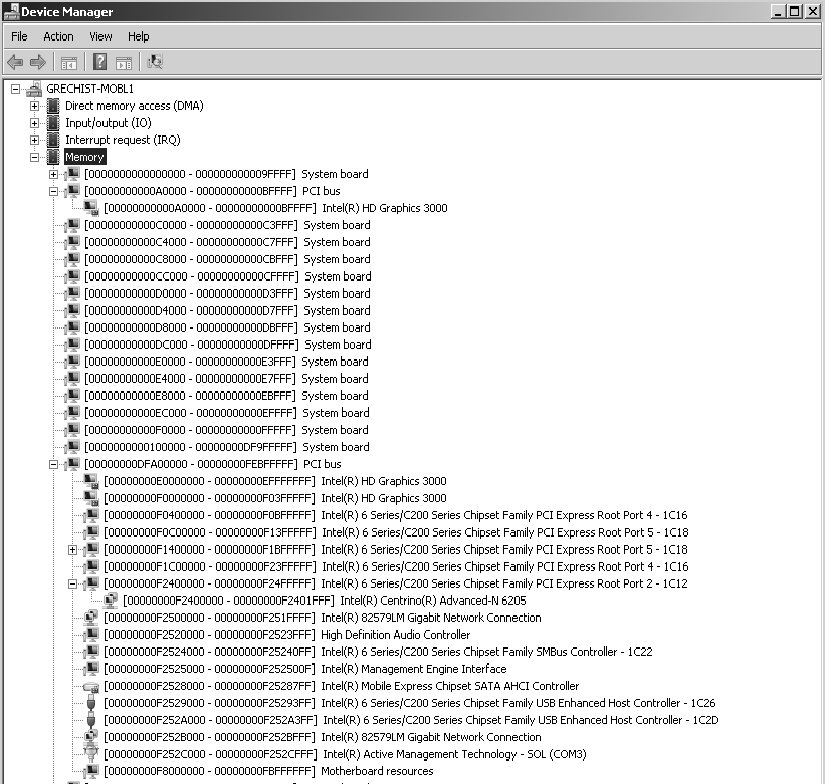
\includegraphics[width=0.9\textwidth]{./memmap-device-manager}
    \caption[Выделение диапазонов памяти в~Windows]{Выделение диапазонов памяти под нужды периферийных устройств в~Windows, наблюдаемое через диспетчер устройств}
    \label{fig:memmap-device-manager}
\end{figure}


\subsection[Карты пространств памяти]{Карты пространств памяти (memory space mappings)}\label{sec:mem-maps}

В реальных сценариях работы функционирование пространств памяти может усложняться следующими обстоятельствами.

\begin{itemize*}
\item Состояние устройств в пространствах памяти может меняться со временем согласно внутренним принципам процесса загрузки системы; количество их регистров также подвержены изменению, их адреса в памяти — тоже.
\item Несколько устройств могут быть расположены в пересекающихся диапазонах адресов, требуя динамического разрешения конфликтов.
\item Одно и то же устройство может одновременно быть расположено по нескольким диапазонам адресов и при этом обеспечивать в них различные побочные эффекты.
\end{itemize*}

Для учёта всех этих особенностей в симуляции используется такая структура, как карта памяти. Для любого доступа по адресу в памяти алгоритм определения устройства, отвечающего за его обработку, следующий~\cite{simics-model-builder-guide} (рис.~\ref{fig:mapalg}).

\begin{figure}[htb]
    \centering
	\inputpicture{drawings/mapalg}
    \caption[Алгоритм поиска устройства в иерархии карт памяти]{Алгоритм поиска устройства в иерархии карт памяти. Перед передачей транзакции доступа конечному устройству её параметры, например адрес, могут быть изменены}
    \label{fig:mapalg}
\end{figure}

\begin{enumerate*}
\item Для доступа определяется его тип (чтение, запись, предвыборка, чтение инструкции и т.п.), адрес начала, длина доступа.
\item В карте памяти по адресу начала определяется нижележащее устройство, которое, в свою очередь, может быть или конечным устройством, или ещё одной картой памяти.
\item Если ни одно устройство не имеет записи в карте, используется устройство по умолчанию (\abbr default target), если оно определено для текущей карты.
\item При необходимости параметры доступа модифицируются так, чтобы соответствовать устройству, например адрес смещается на фиксированную величину.
\item Если полученное устройство — карта памяти, то поиск продолжается в ней, иначе доступ в память передаётся найденному устройству на обработку. 
\item Ситуация, когда для данного адреса не существует трансляции, является ошибкой в конфигурации модели. Также, скорее всего (но необязательно), по конвенциям работы аппаратуры и исполняющейся программы некорректным будет являться многобайтный доступ, части которого попадают в различные устройства.
\end{enumerate*}

Для разрешения неоднозначности при ситуации, когда одно и то же устройство размещено в нескольких картах, в доступе в память из карты добавляется дополнительное число — номер функции. При обработке транзакции устройство может проверить данный номер и скорректировать своё исполнение. Ещё одна задача, которую выполняют с помощью карт памяти — динамическое изменение порядка байт (endianness) доступа, если конечное устройство это требует.

\section{Линии прерываний}

Прерывания являются ещё одним методом коммуникации пери\-фе\-рий\-ных устройств, чаще всего с ЦПУ. Однако, в отличие от рассмотренных ранее способов, оно характеризуется следующими отличиями.

\begin{itemize*}
\item Инициатором взаимодействия является периферийное  уст\-ройст\-во. Процессор в зависимости от ряда условий может отложить обработку полученных прерываний до момента, когда это станет возможным или алгоритмически корректным, или же немедленно перейти в процедуру обработки.

\item Прерывание несёт один бит информации, означающий, что на каком-то из внешних устройств имеется событие, требующее внимания. На каждую линию может быть подключено несколько устройств; в таком случае получатель сигнала прерывания не способен сразу различить, которое из них было инициатором — требуется проинспектировать все из них.

\item Коммуникации однонаправленны в отличие от, например, чтения из регистра, при котором как читающее, так и пишушее устройство имеет возможность получить некоторую информацию о взаимодействии.
\end{itemize*}

% However, it is always treated separately for a number of reasons. It is device-initiated, as opposed to the methods mentioned above, which are CPU-initiated. It is also unidirectional, as information flows only from device to CPU. Lastly, each interrupt line carries only one bit of information with a fixed meaning, namely "an event that requires attention has occurred in a device on this interrupt line".

%Моделирование работы линии прерываний сильно зависит от её архитектурных особенностей. В общем случае оно может быть реализовано как обратный вызов (\abbr callback).

Моделирование работы линии прерываний может быть выполнено следующим способом: в модели архитектурного состояния устройства-получателя заводится флаг \texttt{bool interrupt_raised}, обозначающий, что произошло прерывание. Процессор после каждой исполненной инструкции проверяет состояние этого флага и в случае, когда он выставлен, меняет своё состояние соответствующим образом, при этом сбрасывая флаг в начальное положение. Недостатки данного подхода: 1) обнаружение события прерывания сдвигается на границу между исполнением инструкций, \emph{после} текущей, что не всегда корректно — некоторые прерывания могут отменять текущую инструкцию, не допуская завершения её симуляции; 2) частый опрос флага снижает скорость работы модели. Альтернативный подход: использовать обратный вызов (\abbr callback) — указатель на функцию (метод), непосредственно оперирующий состянием процессора. Инициатор прерывания имеет возможность вызвать указанную функцию для сигнализации прерывания, и затем уже логика работы самого процессора должна определять, в какой момент оно будет им обработано.

\section{Оптимизации при моделировании}

Как было описано выше, достаточно просто обеспечить моделирование состояния с помощью переменных и массивов переменных, хранящихся в памяти. Такое решение универсально и используется во всех случаях. Тем не менее для ускорения работы моделей иногда применимы описанные далее оптимизации.

\subsection{Прямое использование состояния хозяина}

В ряде ситуаций хозяйское оборудование предоставляет аппаратные ресурсы, в том числе и регистры, которые можно переиспользовать для нужд модели, одновременно ускоряя её. Состояние гостевой системы (частично) хранится не в медленной оперативной памяти, а в более быстрых регистрах.

Такой режим работы модели приобретает признаки прямого исполнения. Цикл симуляции при этом имеет следующие стадии.

\begin{itemize*}
\item Гостевое состояние регистров/памяти загружается на соответствующие регистры хозяина.
\item Симуляция проводится в течение некоторого времени.
\item При восстановлении контекста хозяина гостевое состояние сохраняется во внешнюю память.
\end{itemize*}

Как и во всех случаях использования прямого исполнения, выигрыш от него нивелируется необходимостью переключения контекста хозяина и гостя, и поэтому перед его реализацией следует оценить, будет ли польза от достаточно кропотливой работы по включению подобной функциональности в модель. Кроме того, применимость метода сильно зависит от степени соответствия архитектур хозяина и гостя.

\subsection{Кэширование доступов к картам памяти}

Как было показано в п. \ref{sec:mem-maps}, обращение по адресу к физической памяти подразумевает инспектирование одной или более карт для определения адресата. Эта процедура может быть длительной и замедлять моделирование исполняющих устройств. Возможность оптимизации здесь проистекает из наблюдения, что подавляющая часть архитектурных запросов в память оканчиваются в ОЗУ-подобных устройствах, не предоставляющих побочных эффектов. Поэтому сам факт обращения к карте памяти можно отложить или скомбинировать с последующими запросами с помощью кэширования на стороне запрашивающего исполняющего устройства, что позволит ему проводить агрессивные оптимизации своей работы.

Подобная техника должна аккуратно отслеживать изменения в используемых картах памяти. Так, при смене типа устройства, обслуживающего некоторый диапазон пространства адресов, все агенты, имевшие возможность кэшировать его, должны быть уведомлены об этом для обеспечения корректной работы модели.

\subsection{Ленивое вычисление флагов}

Один из типов регистров, встречающихся в современных процессорах — это регистр флагов, каждый бит которого означает, что результат предыдущей операции (как правило, арифметической или логической) имеет определённые свойства. Так, флаг ZF (\abbr zero flag) выставляется в значение 1, если результат предыдущей команды равен нулю, OV (\abbr overflow flag) — если он не может быть сохранён в ограниченном числе двоичных разрядов, отведённых для него, и т.д~\cite{intelmanual1}. Корректное моделирование очень большого числа инструкций подразумевает вычисление и сохранение отдельных битов регистра флагов. Даже для простой операции сложения, результат которой получается с помощью единственной машинной инструкции хозяина, приходится включать длинный блок в десятки инструкций для проверки свойств данного результата.

Общим наблюдением, ведущим к идее следующей оптимизации, является тот факт, что результат, хранящийся в регистре флагов, используется далеко не каждой последующей инструкцией, и потому нет нужды обновлять его так часто. Достаточно производить такую работу только когда это действительно будет необходимо для корректной обработки операции, зависящей от регистра флагов~\cite{bochs}, или при инспектировании состояния пользователем. 

\begin{digression}
В программировании подход (стратегия) вычислений, при котором анализ и исполнение выражения происходит лишь при необходимости использовать его результат, называется \textit{ленивым} (\abbr lazy), в отличие от \textit{энергичного} (\abbr eager) подхода, при котором выражение вычисляется сразу после доступности значений всех его входных слагаемых. % Ленивые вычисления позволяют 
\end{digression}

\section{Точки сохранения}

Возможность сохранения состояния программы в файл с возможностью последующего восстановления и возобновлением работы из него является необходимым для широкого класса приложений: параллельные программы, отказоустойчивые системы, энергосберегающие программы. Для симуляторов наличие такой функциональности означает экономию времени при изучении поведения гостевых систем. Рассмотрим, что должно входить в такую \textit{точку сохранения} (\abbr checkpoint или savepoint).

\begin{itemize*}
    \item Архитектурное состояние всех моделируемых устройств. Если использовались некоторые из описанных выше техник увеличения скорости симуляции, например, размещение состояния на хозяйских регистрах, то необходимо предварительно привести модель в <<стабильный>> режим, когда все подлежащие сохранению регистры имеют гарантированное расположение в памяти.
    
\item    Если часть элементов архитектурного состояния функционально связана с другими элементами, то возможно исключить их из содержимого точки сохранения и пересоздавать их при восстановлении. Это поможет избежать возможности рассинхронизации таких элементов. Состояние программы, не определяющее архитектурное состояние моделей, как правило, не стоит сохранять — это сэкономит время на отладку. К примеру, не стоит дорожить кэшем двоичной трансляции.
    
    \item Информация о соединении моделей отдельных устройств друг с другом. Для различения объектов необходимо использовать некоторые идентификаторы, которые можно будет использовать в качестве ссылок на них в других устройствах при хранении. Такие идентификаторы должны <<переживать>> уничтожение самих объектов с их последующим пересозданием. Поэтому, например, машинные адреса не подходят, так как при перезапуске они каждый раз будут различаться.
\end{itemize*}

\subsection{Переносимость точек сохранения}

Если симулятор планируется использовать на различных хозяйских системах, то необходимо предусмотреть сценарий сохранения гостевого состояния на одной, а восстановление — на другой, и что edianness, разрядность и форматы хранения данных при этом могут различаться. Например, нельзя хранить указатели, так как на другой системе они будут бесполезны.

\subsection[Обращение во времени]{Обращённое во времени исполнение}\label{revexec}

Периодическое сохранение состояния симулируемой системы в сочетании с детерминизмом симулятора позволяет реализовать такой невозможный в реальном мире сценарий исполнения, как обращённое во времени исполнение (\abbr reverse execution), см.~рис.~\ref{fig:reverse-execution}. 

\begin{figure}[htb]
    \centering
	\inputpicture{drawings/reverse-execution}
    \caption{Обращённое во времени исполнение}
    \label{fig:reverse-execution}
\end{figure}

При периоде снятия точек сохранений $T$, текущем времени симуляции $t$  и необходимости откатиться на $\Delta t$ секунд выполняются следующие шаги.

\begin{enumerate*}
    \item Восстановление к точке $t^\star$, ближайшей слева к моменту $t-\Delta t$:
    $$ t^\star = \lfloor (t - \Delta t) / T \rfloor \cdot T. $$
    \item Прямая симуляция до необходимой точки в течение $t_{direct}$:
    $$t_{direct} = t - \Delta t - t^\star .$$
\end{enumerate*}

Поскольку любая симуляция из фиксированного состояния всегда приводит к одинаковому финальному состоянию, то указанная последовательность действий эквивалентна <<скачку>> из момента $t$ в момент $t - \Delta t$.

Постепенно увеличивая значения $\Delta t$, можно создать видимость того, что состояние модели эволюционирует в обратном направлении в симулируемом времени. 

Скорость обращённой симуляции будет обратно линейно зависеть от значения $T$ — чем чаще делаются точки сохранения, тем в среднем короче длина необходимой прямой симуляции. Однако объём памяти, требуемый для хранения всех точек сохранения, также растёт с уменьшением $T$.

\subsection{Миграция}

Процесс возобновления симуляции гостя на хозяйской системе, отличной от той, на которой была создана точка сохранения, получил название <<миграция>>. Возможность миграции важна для распределённых систем виртуализации, призванных обеспечить устойчивость исполнения и минимальный простой виртуальных машин при угрозах отказа аппаратуры физических компьютеров. Если некоторая хозяйская система сигнализирует о сбое из-за отказа жёстких дисков, памяти, питания и т.п., то виртуальные машины, исполнявшиеся до этого на ней, перезапускаются из точек сохранения, регулярно создаваемых и сохраняемых на внешнем хранилище, на оставшихся исправных хозяевах. Наблюдаемое клиентами время простоя сервиса, обеспечиваемого мигрированными виртуальными машинами, минимально.

\subsection[Формат точек сохранения]{Формат файлов точек сохранения}

Не существуют общепринятого соглашения о формате файлов, используемых для сохранения состояния гостевых систем, так как они очень сильно зависят от структуры моделей и особенностей симулятора. Сформулируем некоторые общие принципы их дизайна.

\begin{itemize*}
    \item Файлы могут быть как двоичные, так и текстовые. Хотя первый формат может обеспечить в среднем меньший размер файлов, содержимое его будет нечитаемым для человека, что усложняет отладку симулятора, разработку инструментов для обработки точек. С другой стороны, некоторые данные изначально неудобны для анализа человеком, например, содержимое памяти, дисков и других массивов данных, тогда как представление их в текстовом виде сильно раздувает их объём. Такие данные следует хранить в двоичном виде, а оставшиеся текстовые данные могут быть сжаты архиватором.
    \item Следует предусмотреть возможность использования общепринятых стандартов хранения данных при проектировании нового формата точек сохранения, т.е. не следует <<изобретать велосипед>>. Например, для представления иерархических данных можно использовать XML (\abbr extended markup languange) или JSON. Для хранения однородных массивов данных, используемых для представления состояния жёстких дисков, оперативной памяти и т.п. сущностей существуют форматы QCOW2 или VMDK. Такой шаг повысит удобство конвертации в/из сторонних смуляторов.
    \item Необходимо явно прописывать endianness сохраняемых данных для выбранного формата. Это поможет в дальнейшем при адаптации симулятора для новых гостевых и хозяйских систем.
\end{itemize*}

\subsection{Инкрементальные точки сохранения}

В ситуациях, когда несколько точек сохранения создаются последовательно с некоторым интервалом для одной симуляции, первая из них должна полностью описывать состяние системы, а последующие точки могут опускать часть данных, не изменившихся с предыдущего раза, и содержать только <<дельту>>,  а также ссылку на предыдущую точку. Это позволяет экономить хозяйское дисковое пространство. Особенно сильный выигрыш происходит при хранении образов дисков и памяти.



\section{\Questions к главе \ref{state}} %\label{state-questions}

\subsection*{Вариант 1}

\begin{questions}

\question[3] Какой байт будет расположен первым в памяти на Little Endian системе при записи числа \texttt{0xaabbccdd} в память?
\begin{solution}[1cm]
0xdd
\end{solution}

\question[3] Выберите правильное отношение для фразы <<машинное слово длиной $w$ байт выровнено в памяти по адресу $addr$>>:
\begin{choices}
    \choice $addr \neq 0\ (\mod w)$ (адрес не делится нацело на длину слова),
    \choice $w = 2^k$ и $addr = 2^m$, $k,m \in \mathbb{N}$ (адрес и длина являются степенями двойки),
    \choice $w = 2^k$ и $addr = 2^m$, $k \leq m $ ,$k,m \in \mathbb{N}$ (адрес и длина являются степенями двойки, степень длины меньше степени адреса),
    \correctchoice $addr = 0\ (\mod w)$ (адрес делится нацело на длину слова).
\end{choices}

\question[3] Почему симулятор не имеет права кэшировать регионы гостевой памяти, помеченные как отображённые на устройства?
\begin{solution}[2cm]
В отличие от простой памяти, хранящей данные без изменений, устройство может менять своё состояние и соответственно содержимое регионов памяти на каждом доступе к нему.
\end{solution}

\question[3] Определение понятия <<машинное слово>>.
\begin{solution}[1cm]
Максимальный объём данных, который процессор данной архитектуры способен обработать за одну инструкцию. 
\end{solution}

\question[3] Какой интегральный тип языка Си наиболее удачно использовать для хранения состояния моделируемого регистра шириной 32 бита?
\begin{choices}
    \choice \texttt{int},
    \choice \texttt{unsigned int},
    \correctchoice \texttt{uint32_t},
    \choice зависит от хозяйской системы.
\end{choices}

\end{questions}

\subsection*{Вариант 2}

\begin{questions}

\question[3] Какой байт будет расположен первым в памяти на Big Endian системе при записи числа \texttt{0xbaadc0de} в память?
\begin{solution}[1cm]
0xba
\end{solution}


\question[3] Какую стратегию подразумевает концепция ленивого вычисления?
\begin{choices}
    \choice Замена точного значения выражения приближённым, но получаемым за меньшее время.
    \correctchoice Запуск вычисления выражения происходит лишь при необходимости использовать его результат.
    \choice Выражение вычисляется сразу после доступности значений всех его входных слагаемых.
    \choice Значение подвыражения, используемого в нескольких других выражениях, сохраняется при первом вычислении и затем переиспользуется.
\end{choices}

\question[3] Определение понятия <<байт>>.
\begin{solution}[1cm]
Минимальная адресуемая в данной архитектуре единица информации.
\end{solution}

\question[3] Сколько бит информации получает процессор при первоначальном возникновении сигнала на линии прерывания?
\begin{choices}
    \correctchoice 1 бит.
    \choice 8 бит.
    \choice Зависит от архитектуры.
\end{choices}

\question[3] Выберите правильные окончания фразы: карта памяти
\begin{choices}
    \correctchoice использует цель по умолчанию, если обрабатываемый запрос не попадает ни в одно из устройств,
    \choice может указывать на устройство не более одного раза,
    \choice должна указывать на все присутствующие в гостевой системе устройства,
    \correctchoice может указывать не только на устройства, но и на другие карты памяти.
\end{choices}


\end{questions}

% К каждой лекции должно быть от 8 до 12 задач, у каждой задачи должно быть 3-5 вариантов формулировок примерно одинаковой сложности. Допускается объединение нескольких последовательных лекций в одну тему и подготовка тестов к темам.
% Задачи должны полностью соответствовать материалам лекций, то есть лекциях должно быть достаточно информации для ответа на все вопросы.
% Формулировка каждого варианта задачи должна содержать всю необходимую информацию и не должна ссылаться на тексты внутри лекции, картинки или другие задачи или варианты задачи.
% Правильные ответы выделяются знаком «+» перед их формулировкой. Правильных ответов может быть несколько. Для тестов с несколькими ответами как минимум один ответ должен быть правильным и как минимум один ответ должен быть неправильным. 
% 
% Структура теста к лекции
% 
% \subsection*{Задача 1}
% 
% \paragraph{Вариант 1} 
% 
%     Чему равно 2+2?
%         Ответ 1. 3
%         + Ответ 2. 4
%         …
%         Ответ N. 5
% \paragraph{Вариант 2}
%     Чему равно 2*2?
%         + Ответ 1. 4
%         + Ответ 2. 2+2
%         …
%         Ответ N. 5
% \paragraph{Вариант 3}
% 
%     Чему равно 2-2?
%         Ответ 1. 0
% 
% 
%         
% \section{Просто подборка вопросов}
% 


 
 
 
\iftoggle{webpaper}{
    \printbibliography[title={Литература}]
}{}


